\section{Methodology}
\label{sec:methods}
% Draft for the authors to review and rewrite in their own words.
% All settings below match the committed code (tag v1.0-results).

Fig.~\ref{fig:pipeline} summarises the approach. Every test image is passed
through the same frozen feature extractor; the methods differ only in the
reference against which each patch is compared. We then evaluate the
anomaly maps with one metric code, analyse how per-image accuracy depends on
defect size, and test the cause with interventions on the reference.

\begin{figure*}[t]
\centering
% Vector figure built from figures/method_overview.tex (see method_overview_standalone.tex)
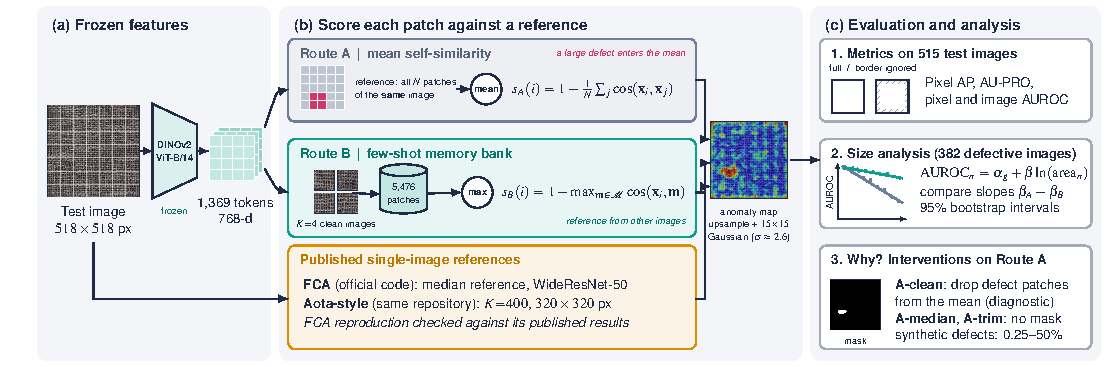
\includegraphics[width=\textwidth]{method_overview.pdf}
\caption{Overview of the methodology. (a)~Each test image is encoded once by a
frozen DINOv2 ViT-B/14 into 1{,}369 patch tokens. (b)~Each patch is scored
against a reference: Route~A uses all patches of the same image, so a large
defect enters its mean; Route~B uses a memory bank built from four clean images;
FCA runs with its official code and the Aota-style variant with the
reimplementation in the same repository, each with its own features. (c)~All anomaly maps are evaluated with one metric code on two
protocols, per-image accuracy is regressed on log defect area, and
interventions on Route~A's reference test the cause. The thumbnails show a
carpet test image, its ground-truth mask and its Route~A map; the reference
tiles are illustrative.}
\label{fig:pipeline}
\end{figure*}

\subsection{Dataset and evaluation protocol}
We use the five texture categories of MVTec AD~\cite{bergmann2021mvtec}:
carpet, grid, leather, tile and wood, with 117, 78, 124, 117 and 79 test
images (515 in total: 133 defect-free and 382 defective). Thirty training
images per category are loaded from the official training split; they serve
only as the pool for Route~B's references. Images are resized to
$518\times518$ pixels.

We report four metrics per texture and their five-texture average:
pixel-level average precision (Pixel AP), the area under the per-region
overlap curve (AU-PRO; 1{,}000 thresholds, integrated up to a false-positive
rate of 0.3 and normalised), pixel AUROC, and image AUROC, for which the
image score is the maximum of the anomaly map. Aota et~al.~\cite{aota2023zeroshot} evaluate on a centre crop that removes
about 10\% of each side, so every result is reported on two protocols: the full image, and a cropped protocol
that ignores a 52-pixel border (about 10\%) of both the map and the mask. Two
defective images (one in grid, one in tile) have their defect entirely inside
this border; they are dropped from the cropped size analysis ($n=380$).

\subsection{Feature extraction}
Both routes use DINOv2 ViT-B/14~\cite{oquab2024dinov2} without any training.
A $518\times518$ input gives a $37\times37$ grid of $N=1{,}369$ patch
tokens of dimension 768, taken from the final block, stored at half precision (fp16) and
L2-normalised. Each
patch score map is upsampled bilinearly to $518\times518$ and smoothed with a
$15\times15$ Gaussian filter (OpenCV, with $\sigma$ derived from the kernel
size, about 2.6 pixels). The main results use the final block; a sweep over
blocks 6, 8, 10, 12 and the mean of blocks 7--9 tests this choice.

\subsection{Route A: single-image mean similarity}
Route~A compares each patch $\mathbf{x}_i$ with all patches of the same
image and uses the mean cosine similarity as its reference:
\begin{equation}
  s_A(i) = 1 - \frac{1}{N}\sum_{j=1}^{N} \cos(\mathbf{x}_i,\mathbf{x}_j).
  \label{eq:routeA}
\end{equation}
A patch that differs from the image as a whole receives a high score. If a
defect covers a large share of the image, however, the defect patches enter
the mean in~\eqref{eq:routeA} and pull the reference towards the defect; this
is the contamination we test in Section~\ref{sec:interventions}.

\subsection{Route B: few-shot memory bank}
Route~B follows the memory-bank idea of AnomalyDINO~\cite{damm2025anomalydino}.
The memory bank $\mathcal{M}$ holds the $4\times1{,}369=5{,}476$ patches of
$K=4$ defect-free reference images, drawn at random by seed from the 30
loaded training images. Each test patch is scored by its distance to the
nearest entry:
\begin{equation}
  s_B(i) = 1 - \max_{\mathbf{m}\in\mathcal{M}} \cos(\mathbf{x}_i,\mathbf{m}).
  \label{eq:routeB}
\end{equation}
Because the reference comes from other images, a defect in the test image
cannot contaminate it. The main results use seeds 42, 123 and 2026. The size analysis
uses seed 42, the interventions on real defects use the mean of ten seeds,
and the synthetic experiments use five seeds. Route~B differs from AnomalyDINO in backbone
size, resolution, smoothing, the absence of rotation augmentation and the
image-level score, so we do not call it AnomalyDINO.

\subsection{Published single-image references}
To test whether any size dependence is specific to Route~A, we run the
official FCA code~\cite{ardelean2024highfidelity} (commit \texttt{afe8326},
MIT licence) at full resolution. Before computing any new result we checked
the reproduction: the published per-texture PRO and pixel AUROC are matched
within 0.01 points on all five textures. The repository pins Python 3.9 and
PyTorch 2.1.2; we ran it with Python 3.13 and PyTorch 2.6.0, with two small
wrapper fixes for file input and output and no change to the method. We also run the repository's
reimplementation of Aota et~al.~\cite{aota2023zeroshot} at $320\times320$
pixels with a $3\times3$ tile and $K=400$. Both sets of maps are rescaled to
the $518\times518$ grid and scored with our metric code.

\subsection{Size analysis}
For each defective image $n$ we compute its pixel AUROC, which does not
depend on how many pixels are defective, and regress it on the natural
logarithm of the defect area (pixels on the $518\times518$ grid):
\begin{equation}
  \mathrm{AUROC}_n = \alpha_{g(n)} + \beta \ln(\mathrm{area}_n) + \varepsilon_n ,
  \label{eq:slope}
\end{equation}
where $\alpha_{g(n)}$ is a fixed effect for each texture--defect-type group
(25 groups), so that the slope $\beta$ is estimated within groups. One unit
of $\ln(\mathrm{area})$ corresponds to multiplying the area by $e\approx2.7$,
and $\beta$ is expressed in AUROC points per unit. A more negative slope means
that accuracy falls faster as defects grow. We compare methods through the
slope difference on the same images (for example $\beta_A-\beta_B$), with
95\% confidence intervals from 10{,}000 bootstrap resamples of images. To
check that a smaller slope is not only a ceiling effect near an AUROC of
100, we also regress the log ratio of the two methods' errors
($100-\mathrm{AUROC}$) on log area.

\subsection{Interventions on the reference}
\label{sec:interventions}
To test whether the defect contaminates Route~A's reference, we change only
the reference in~\eqref{eq:routeA}:
\begin{itemize}
  \item \textbf{A-clean} takes the mean over non-defect patches only, using
  the ground-truth mask. It is a diagnostic, not a deployable method.
  \item \textbf{A-median} replaces the mean by the median of the similarities.
  \item \textbf{A-trim} replaces it by a mean that drops the lowest 25\% of
  the similarities.
\end{itemize}
If contamination drives the size dependence, A-clean should remove much of
Route~A's slope, while the two mask-free variants show how much a simple
robust statistic recovers. We also compute a contamination index, the
distance between the mean feature of the whole image and the mean feature of
its non-defect patches.

\subsection{Synthetic defects}
Real defects do not allow size to be varied independently of content.
We therefore paste synthetic defects into the 133 defect-free test images:
irregular single-component blobs filled with a crop of another texture,
Gaussian noise ($\sigma=8$ grey levels), blur ($\sigma=8$ pixels) or a hue
shift of $60^\circ$ with brightness reduced to 65\% (on the greyscale grid
images only the darkening applies), at ten area fractions from 0.25\% to
50\%. Bootstrap resampling is over the 133 base images, because the copies of
one image are not independent. The key test compares 25\% with 50\% coverage:
once the defect is half of the image, a contaminated mean reference should
fail, while A-clean should not.

\subsection{Pre-set criteria and implementation}
For each analysis we fixed the success criterion before running it, and we
report every outcome, including negative ones. Two deviations are disclosed:
the 25\% coverage was added in a second run, because the first sweep
contained 32\% but not 25\% (in that first sweep the test held against 32\%
but not against 0.25\%, and we report both); and the drift criterion did not
specify the expected sign of its coefficient: drift met it, but with the
opposite sign to our hypothesis, so we do not treat drift as a mechanism. All experiments ran on a laptop with an
NVIDIA RTX 3050 GPU (4~GB), Python 3.13, PyTorch 2.6.0 and CUDA 12.4. Code,
configuration and results are kept in a git repository (release tag
\texttt{v1.0-results}).
